\section{System design}
In this chapter, the design of the system is explained.
The focus of section 3.1 will be an overview of the first approach implemented, the ring topology. Here, a detailed analysis of this architecture and its trade-offs is presented. However, due to the issues and complexities described below, it was discarded and not finished. Subsequently, in section 3.2 there is an analysis of the second approach, the implemented one, where components have full connectivity. Lastly, in section 3.3 we discuss the additional features implemented in the system.

\subsection{Ring topology}

The proposed architecture, shown in figure 1, consists on a logical ring of GSs and evenly divided groups of RMs.
Each group of RMs is monitored by one GS (blue lines on the figure), being monitored means that the GS oversees the execution of the workloads conducted at those clusters. Thus, periodically, RMs ping the monitoring GS indicating they are alive and what current load of the cluster is. Additionally, each group of RMs is backed up by the next GS in the ring (red lines on the figure) thus, RMs also ping the back-up GS periodically. The role of the back-up GS is to supervise the RMs and take action in case of failure. Apart from that, every GS exchange information about the clusters under its supervision with the next and previous GS of the logical ring (black lines).
\\ 
\begin{figure}[H]
\centering
	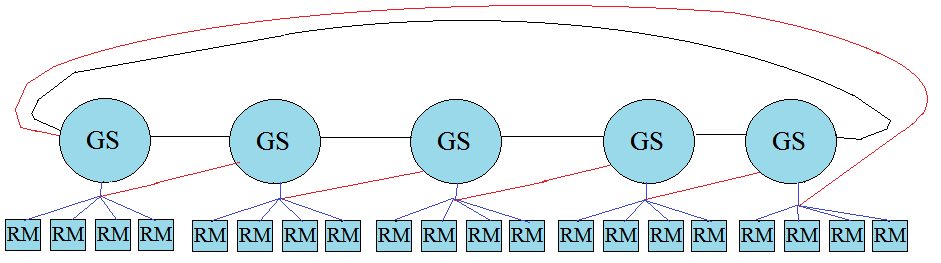
\includegraphics[scale=0.61]{ring.png}
	\caption{Ring topology}
\end{figure}

\subsubsection{Initialization}
Since the topology is fixed, the components need to know in advance with whom they are going to be connected to, which makes initialization hard and complex.

\subsubsection{Workflow}
When a job request arrives at an RM this will decide either to queue or to offload the request based on the current load. 
In case that there are resources available to attend the request, the RM will first send the job to both, monitoring and back-up GS for replication. Once the replication requests have been acknowledged, the user will be notified that the her job has been accepted and that it will be queued for execution. Otherwise, the job is sent to the monitoring GS, which will handle the allocation of the job.
\\\\
The job is executed by the first node which becomes available. Upon completion of the execution, the RM informs the monitoring and back-up GS that the monitoring resources allocated for that job request can be released. A diagram of the workflow is displayed on the figure 2 below.
\\
\begin{figure}[H]
\centering
	\includegraphics[scale=0.45]{workflow.png}
	\caption{Workflow in the ring topology}
\end{figure}

\paragraph{Fault recovery}
RMs and GSs may fail at any time and restart, failures are discovered due to ping timeout. When a monitoring GS notices that one of the RMs under its supervision has failed, it will inform the back-up GS to stop monitoring the crashed RM. Immediately after that, it will reallocate the jobs which were executing in the failed RM to a new cluster. Once the new RM receives the workload from the GS, it will proceed with the replication and scheduling as in the normal workflow. On the other hand, when a back-up GS detects the failure of the monitoring GS, it will promote itself to become the monitor of the clusters supervised by the crashed GS. Subsequently, the RM will connect to the next GS on the ring, next to the failed one, as backup GS. The action flow in the case of back-up GS crash is rather similar, the RM will connect to the next GS in the ring as back-up.
\\\\
This strategy of fault recovery may seem robust, however, it is likely to trigger a failure of the whole system due to a domino effect in the fault recovery. The reason behind that is that all the workload monitored by a failed GS is entirely supported by the back-up. If the latter is already heavy loaded, it will probably fail as well, triggering a cascade failure. This scenario is also possible in the case of an RM failure, the GS monitoring the new selected cluster will assume all the incoming workload. Without a protocol to re-balance the topology when a component resumes its activity, all RMs will eventually be monitored by a single GS.

\paragraph{Load balance}
As a response to the pings, GSs receive the load of the clusters they monitor, this load is then propagated around the ring in both directions. In this way, when a GS receives a job offloaded by an RM it can easily choose a new cluster trying to balance the load of the whole system. The way of selecting the new RM is by using an inverted weighed random selection with the load of each cluster.

\subsubsection{Scalability}
Adding a new GS will only imply connecting the new component to another two GSs and two RMs (one as main monitoring and one as back-up). Similarly, an extra RM will just ping a main GS and a back-up GS. Thus the topology does not present message overload and scales with $O(1)$.

\subsubsection{Issues}
In this topology each component has dependencies on specific other components, making the initialization of the system difficult. Moreover, when failures occur, the topology of the system changes. In order to re-balance the new topology, a protocol for joining the system would be needed, which adds significant more complexity. Despite the fact that this topology was designed to be resilient against failures, domino failures may kill the whole system, as discussed above. Considering these issues, the described approach does not seem adequate.

\subsection{Fully connected topology}
Given the issues of the ring topology described above, we chose to implement a second approach, described in the remainder of this subsection.
To circumvent said issues, in this solution GSs are fully connected among themselves and RMs ping all GSs present in the system. A diagram of the topology is shown in figure 3 below.

\begin{figure}[H]
\centering
	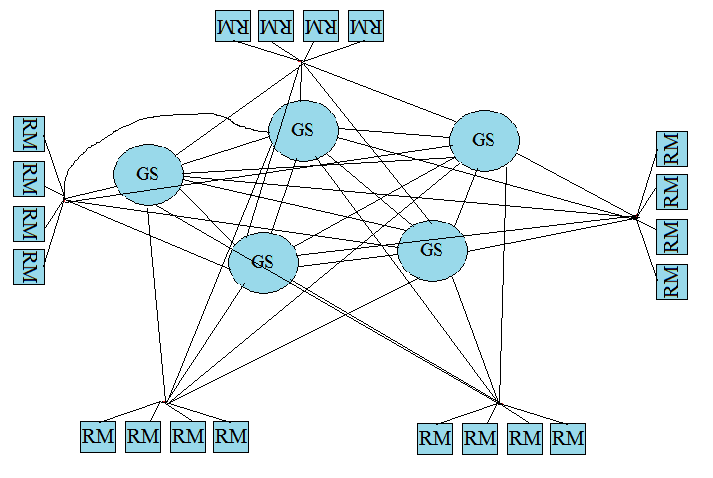
\includegraphics[scale=0.51]{full.png}
	\caption{Fully connected topology}
\end{figure}

\subsubsection{Initialization}
All the components have a list of URLs of the whole system, once started they begin to ping periodically each other. Each RM is ready to serve requests once it is connected to at least two GSs.

\subsubsection{Workflow}
To account for the changed topology, some changes have been made regarding the workflow. Once a job requests arrives at an RM, a monitoring and back-up GS are chosen randomly among all the GSs of the system. When an RM needs to offload a job request, it also selects randomly the GS to offload the job to. Similarly to the ring topology, the chosen GS will allocate the job to an RM which will take care of the execution.

\paragraph{Fault recovery}
Failure detection is detected in the same manner as in the ring topology. However, because the monitoring and back-up selection is made randomly for each job request, it is unlikely to trigger a domino failure, making the system more robust. Also, when a crashed component resumes its activity, it will simply notify the rest of the system so it can be selected again for monitoring/back-up (in the case of a GS) or processing job requests in the case of an RM. Another improvement compared to the ring topology is the tolerance against multiples crashes. Single failures of GSs are handled in the same way than in the ring topology, however the way of handling RM crashes is slightly different. In this setup, once the monitoring GS notices that an RM has crashed, it will reallocate all the jobs in another RM but, since there are no fixed GS assigned to any RM, the monitoring GS will also monitor these jobs during their execution in the new selected RM. Thus, the new RM will only request a new back-up GS before scheduling the jobs. Another important difference is that the selection of the new RM is done for each of the jobs present in the failed RM, since the new RM is chosen by using an inverted weighed random selection, it is extremely unlikely that a single RM receives all the workload of the failed one, reducing the possibility of cascade failure.
\\\\
In the case of a simultaneous crash of an RM and its monitoring GS, the back-up will promote itself to become the monitoring GS of the workload of the failed RM. After that, the recovery process is identical to the case of a single RM crash. Similarly, if the back-up GS and RM crash at the same time, the recovery process is conducted by the survival monitoring GS, it will reallocate the jobs in new RMs, which will select new back-ups. Lastly, if both GSs fail simultaneously, the RM will select a new monitor and back-up before continuing its activity.

\paragraph{Load balance}
The load balancing process is exactly the same than in the ring topology, however, because every RM pings every GS, the retransmission of the messages with load among GSs is not needed.

\subsubsection{Scalability}
This topology scales with $O(|GS|\cdot |GS|-1 + |RM|\cdot |GS|) = O(n^2)$. Where $|GS|$ and $|RM|$ denote the number of GSs and RMs respectively. The first term $|GS|\cdot |GS|-1$ is the number of messages among GSs, whereas the second term $|RM|\cdot |GS|$ indicates the number of messages between RM and GS. This scalability factor clearly is not good, however, taking into account that the size of the pings is extremely small, as they just contain the load of the clusters, the total overload is not too high.

\subsection{Additional features}
As explained above, the system designed is able to tolerate failures in at most two nodes at the same time. Actually, it can tolerate multiple combinations of failures in GS/RM as long as there are components nodes to support the total workload of the system. Going beyond what it was previously said, the system has the ability to deal simultaneously with diverse users since job requests include a user identifier. As it will be shown in the experiments section, the different workloads are treated evenly, in this way the system offers an equitative service.